\documentclass[10pt,a4paper]{article}
\usepackage[utf8]{inputenc} %extra characters
\usepackage[ngerman]{babel} %deutsche Spracheinstellung
\usepackage{blindtext} %generiert zufälligen Text
\usepackage{amsmath,amssymb} % erleichtert Mathe 
\usepackage{enumerate} % schicke Nummerierung
\usepackage{enumitem} %römische/alphabetische Nummerierung
\usepackage{graphicx} % für Grafik-Einbindung
\usepackage{framed}
\usepackage{xcolor}
\usepackage{mdframed}
\usepackage{hyperref}
\usepackage[backend=biber,style=numeric,]{biblatex}
\hypersetup{
colorlinks=true, %set true if you want colored links
linktoc=all,        %set to all if you want both sections and subsections linked
linkcolor=blue,   %choose some color if you want links to stand out
citecolor=blue,	%choose chite color
urlcolor = blue	%url color
}
\addbibresource{literatur.bib}

\usepackage{fancyhdr}
\lhead{Banachräume}
\chead{}
\rhead{Patrick Müller}
%\renewcommand{\headrulewidth}{0.4pt}
%\renewcommand{\footrulewidth}{0pt}
\fancyheadoffset[loh,reh]{3mm}
\fancyhf[cf]{\thepage}



%%%%%%%%%%%%%%%%%%%%%%%%%%%%%%%%%%%%%%%%%%%%%%%%%%%%%%%%%%%%%%%%%%
%
%  geometry
%
\usepackage{geometry}
\geometry{top=2cm,bottom=2cm,left=2.5cm,right=2.5cm}
%
% Ende geometry
%
%%%%%%%%%%%%%%%%%%%%%%%%%%%%%%%%%%%%%%%%%%%%%%%%%%%%%%%%%%%%%%%%%%

%%%%%%%%%%%%%%%%%%%%%%%%%%%%%%%%%%%%%%%%%%%%%%%%%%%%%%%%%%%%%%%%%%
%
%  ntheorem
%
\usepackage[thmmarks,amsmath,hyperref,noconfig]{ntheorem} 
% erlaubt es, Sätze, Definitionen etc. einfach durchzunummerieren.
\theorembodyfont{\upshape}
\colorlet{shadecolor}{blue!15}

\theoremstyle{plain}
\newtheorem{satz}{Satz}[section]
\newenvironment{sa}{\begin{shaded}\begin{satz}}{\end{satz}\end{shaded}}
\theoremstyle{definition}
\newtheorem{hilfssatz}[satz]{Hilfssatz}
\newenvironment{hsa}{\begin{hilfssatz}}{\end{hilfssatz}}
\newtheorem{korollar}[satz]{Korollar}
\newenvironment{kor}{\begin{korollar}}{\end{korollar}}
\newtheorem{definition}[satz]{Definition}
\newenvironment{dfi}{\begin{shaded}\begin{definition}}{\end{definition}\end{shaded}}
\newtheorem{folgerung}[satz]{Folgerung}
\newenvironment{fol}{\begin{shaded}\begin{folgerung}}{\end{folgerung}\end{shaded}}
\newtheorem{lemma}[satz]{Lemma}
\newenvironment{lem}{\begin{shaded}\begin{lemma}}{\end{lemma}\end{shaded}}

\theoremstyle{nonumberplain}
\newtheorem{beispiel}{Beispiel}
\newenvironment{bsp}{\begin{beispiel}}{\end{beispiel}}
\newtheorem{bemerkung}{Bemerkung}
\newenvironment{bem}{\begin{bemerkung}}{\end{bemerkung}}
\theoremsymbol{\ensuremath{_\square}}
\newtheorem{beweis}{Beweis}
\newenvironment{bew}{\begin{beweis}}{\end{beweis}}
\qedsymbol{\ensuremath{_\square}}
%\theoremclass{LaTeX}
%
% Ende ntheorem
%
%%%%%%%%%%%%%%%%%%%%%%%%%%%%%%%%%%%%%%%%%%%%%%%%%%%%%%%%%%%%%%%%%%

%%%%%%%%%%%%%%%%%%%%%%%%%%%%%%%%%%%%%%%%%%%%%%%%%%%%%%%%%%%%%%%%%%
%
% shortcuts
%
\DeclareMathOperator{\GL}{GL} % einige Macro, siehe am Ende Abschn. 2
\newcommand{\N}{\mathbb{N}}
\newcommand{\Z}{\mathbb{Z}}
\newcommand{\Q}{\mathbb{Q}}
\newcommand{\R}{\mathbb{R}}
\newcommand{\C}{\mathbb{C}}
\newcommand{\cP}{{\mathcal P}} 
\newcommand{\K}{\mathbb{K}}
\newcommand{\RM}[1]{\MakeUppercase{\romannumeral #1{.}}} %römische Zahlen
%
% Ende shortcuts
%
%%%%%%%%%%%%%%%%%%%%%%%%%%%%%%%%%%%%%%%%%%%%%%%%%%%%%%%%%%%%%%%%%%
\begin{document}
\renewcommand{\figurename}{Abb.}
%Deckblatt
\begin{titlepage}
	\centering
	{\Large\bfseries Patrick Müller \par}
	\vspace{5cm}
	{\huge\bfseries Banachräume\par}
	\vspace{1cm}
	{\scshape\Large\bfseries Mathematisches Seminar\par}
	\vspace{1cm}
	{\Large Wintersemester 2022\par}
	\vspace{2cm}
	\large\today
	\vspace{7cm}

	\vfill
    
\includegraphics[width=0.45\textwidth]{pictures/thws.png}\par\vspace{1cm}
	\vfill
\end{titlepage}

%Leere Seite
%\setcounter{page}{2}
%\newpage 
%\thispagestyle{empty}
%\quad 
%\newpage

%Inhalsverzeichniss
\renewcommand*\contentsname{Inhalt}
\tableofcontents{}
\newpage
\pagestyle{fancy}
%%%%%%%%%%%%%%%%%%%%%%%%%%%%%%%%%%%%%%%%%%%%%%%%%%%%%%%%%%%%%%%%%%
%Einleitung
%%%%%%%%%%%%%%%%%%%%%%%%%%%%%%%%%%%%%%%%%%%%%%%%%%%%%%%%%%%%%%%%%%
\section*{Einleitung}
\addcontentsline{toc}{section}{Einleitung}
In der Analysis gibt es eine Vielzahl an Räumen. Alle diese Räume haben mathematische Objekte mit bestimmten Strukturen zugrundeliegen. Durch deren charakteristische Beziehungen und Strukturen können Räume unterschiedlichste Eigenschaften besitzen. Ein paar dieser Eigenschaften interessieren uns besonders. \\\\Anfangs werden grundlegende Konzepte aus der Linearen Algebra und der Analysis wiederholt, die es uns ermöglichen, weitere Eigenschaften zu definieren. Hierbei dient uns vor allem das Konzept eines Vektorraums als algebraische Voraussetzung, womit wir die Norm und auch anschließend die Konvergenz in normierten Räumen  einführen können. \\\\Das führt uns dann zu einer der wohl wichtigsten Raumeigenschaften, nähmlich der Vollständigkeit. Die Vollständigkeit kann normierte Vektorräume zu sogenannten Banachräumen machen. Da in der Funktionalanalysis auch hauptsächlich unendlichdimensionale Räume untersucht werden, betrachten wir anschließend einen vollstänidgen Funktionenraum und einen vollstänidgen Folgenraum jeweils genauer. Auch andere wichtige Eigenschaften aus der Topologie, wie z.B. Abgeschlossenheit, Separabilität oder auch das wichtige Konzept der Kompaktheit, werden genauer bearbeitet.  \\\\Am Ende schauen wir uns dann noch zwei zentrale Sätze der Funktionalanalysis an. Einer dieser Sätze, ist der Satz von Baire, mit dem sich elegante Beweise im Bereich der Funktionalanalysis führen lassen. So lässt sich z.B. der Satz von Banach-Steinhaus, das Prinzip der gleichmäßigen Beschränktheit oder auch der Satz über die offene Abbildung, aus dem Satz von Baire ableiten.\\ Ein weiterer wichtiger Satz ist der Satz von Heine-Borel. Dieser Satz stellt einen elementaren Bezug zwischen Kompaktheit und Abgeschlossenheit her. Im Folgenden werden wir zwei Varianten dieses Satzes kennenlernen, da sich dieser Satz zum einen für Teilmengen des $\R^n$, aber zum anderen auch allgemein für metrische Räume formulieren lässt. \\\\Bei dem Thema Banachräume interessieren wir uns hauptsächlich für normierte Räume, jedoch lassen sich viele Aussagen auch allgemeiner auf metrischen Räumen treffen. Darauf wird auch in dieser Arbeit nicht verzichtet, sodass einige Definitionen und Sätze über metrische Räume formuliert werden.
\newpage

%%%%%%%%%%%%%%%%%%%%%%%%%%%%%%%%%%%%%%%%%%%%%%%%%%%%%%%%%%%%%%%%%%
%Grundlagen
%%%%%%%%%%%%%%%%%%%%%%%%%%%%%%%%%%%%%%%%%%%%%%%%%%%%%%%%%%%%%%%%%%
\section{Grundlagen}
%%%%%%%%%%%%%%%%%%%%%%%%%%%%%%%%%
%Vektorraum
%%%%%%%%%%%%%%%%%%%%%%%%%%%%%%%%%
\subsection{Vektorraum}

Ein Vektorraum oder linearer Raum ist eine algebraische Struktur, die in vielen Teilgebieten der Mathematik verwendet wird. Vektorräume bilden den zentralen Untersuchungsgegenstand der linearen Algebra und sind auch grundlegend für die Funktionalanalysis. Sie können addiert oder mit Skalaren multipliziert werden. Das Ergebnis ist wieder ein Vektor des selben Vektorraums.
\begin{dfi}
\label{vektorraum}
(vgl. Ref. \cite{Fischer}, S.76) Sei $\K$ ein Körper. Eine nichtleere Menge $V$ zusammen mit einer inneren Verknüpfung
\begin{align*}
+ : V \times V \rightarrow V, \enspace (v, w) \mapsto v + w \enspace \text{(Addition)}
\end{align*}
und einer äußeren Verknüpfung
\begin{align*}
\cdot : \K \times V \rightarrow V, \enspace (\lambda, v) \mapsto \lambda \cdot v \enspace \text{(Skalarmultiplikation)}
\end{align*}
heißt $\K$-\textit{Vektorraum}, wenn Folgendes gilt:
\begin{enumerate}[label=(\roman*)]
\item $V$ bildet zusammen mit der Addition + eine \textit{abelsche Gruppe} und erfüllt die Axiome:
\begin{enumerate}[label=(\arabic*)]
\item $v + (w + z) = (v + w) + z$ für alle $v,w,z \in V$ (Assoziativgesetz)
\item $v + w = w + v$ für alle $v,w \in V$ (Kommutativgesetz)
\item Es gibt ein Element $0 \in V$, so dass für alle $v \in V$ gilt: $v + 0 = v$. Dieser Vektor $0$ heißt \textit{neutrales Element} oder auch \textit{Nullvektor}. (Existenz neutrales Element)
\item Zu jedem $v \in V$ gibt es ein $y \in V$, so dass gilt: $v + y = 0$. $y$ heißt inverses Element zu $v$. Statt $y$ schreiben wir auch $-v$. (Existenz inverses Element)
\end{enumerate}
\item Zusätzlich müssen folgende Axiome der Skalarmultiplikation $\cdot$ erfüllt sein:
\begin{enumerate}[label=(\arabic*)]
\item $(\lambda + \rho) \cdot v = (\lambda \cdot v) + (\rho \cdot v)$ für alle $\lambda,\rho \in \K, v \in V$ (Skalares Distributivgesetz)
\item $ \lambda \cdot (v + w) = (\lambda \cdot v) + (\lambda \cdot w)$ für alle $\lambda \in \K, v,w \in V$ (Vektor Distributivgesetz)
\item $(\lambda \cdot \rho) \cdot v = \lambda \cdot (\rho \cdot v)$ für alle $\lambda,\rho \in \K, v \in V$ (Skalares Assoziativgesetz)
\item Für alle $v \in V$ und für $1 \in \K$ gilt: $1 \cdot v = v$. 1 heißt \textit{neutrales Element der Skalarmultiplikation}. (Neutrales Element der Skalarmultiplikation)
\end{enumerate}
\end{enumerate}
\end{dfi}
\begin{bem}
Anstelle von $V$ schreibt man auch oft $(V,+,\cdot)$. 
\end{bem}
\begin{dfi}
\label{unterraum}
(vgl. Ref. \cite{Fischer}, S.77) Sei $V$ ein $\K$-Vektorraum und $U \subset V$. Dann heißt $U$ \textit{Unterraum} von $V$, falls Folgendes gilt:
\begin{enumerate}[label=(\roman*)]
\item $U \neq \emptyset$
\item $v,w \in U \Rightarrow v + w \in U$ (Abgeschlossen bezüglich der Addition)
\item $v \in U, \lambda \in \K \Rightarrow \lambda v \in U$ (Abgeschlossen bezüglich der Skalarmultiplikation)
\end{enumerate}
\end{dfi}
Im Folgenden werden wir uns auf die Fälle $\K = \R$ oder $\K = \C$ beschränken.
\newpage
%%%%%%%%%%%%%%%%%%%%%%%%%%%%%%%%%
%Metrische Räume
%%%%%%%%%%%%%%%%%%%%%%%%%%%%%%%%%
\subsection{Metrische Räume}

Eine Metrik ist eine Funktion, die je zwei Elemente einer Menge einem nichtnegativen reellen Wert zuordnet. Sie definiert einen Abstandsbegriff und bringt damit eine triviale Struktur auf eine Menge. Wie wir später sehen werden, ist es mit Hilfe dieser Struktur möglich weitreichende allgemeine Aussagen zu treffen.
\label{metrik}
\begin{dfi}
(vgl. Ref. \cite{Forster}, S.3): Sei $X$ eine Menge.  Eine \textit{Metrik} auf $X$ ist eine Abbildung $d : X \times X \rightarrow {\R_0}^+$, die für alle $x, y, z \in X$ folgenden Eigenschaften erfüllt:
\begin{enumerate}[label=(\roman*)]
\item $d(x, y) = 0 \Leftrightarrow x = y$ (Nichtdegeneriertheit)
\item $d(x, y) = d(y, x)$ (Symmetrie)
\item $d(x, z) \leq d(x, y) + d(y, z)$ (Dreiecksungleichung)
\end{enumerate}
Versieht man die Menge $X$ mit einer Metrik $d$, so bildet das Paar $(X, d)$ einen \textit{metrischen Raum}, wobei $d(x,y)$ einen Abstand zwischen den zwei Punkten $x$ und $y$ definiert.
\end{dfi}
\begin{bem}
Zu beachten ist hier vor allem, dass noch keine algebraische Struktur gefordert ist und somit noch keine Möglichkeit besteht, Differenzen von Elementen zu bilden. Desweiteren lässt sich aus den Axiomen der Metrik folgern, dass eine Metrik stets nicht negativ ist und somit für alle $x,y \in X$ gelten muss: $d(x,y) \geq 0$.
\end{bem}
\begin{bew}
Wendet man die Dreiecksungleichung auf die Punkte $x, y, x$ an, so folgt unter Verwendung von (i) und (ii):  $0 = d(x, x) \leq d(x, y) + d(y, x) = 2d(x, y)$
\end{bew}
\begin{bsp}
(vgl. Ref. \cite{Clason}, Beispiel S.4) Klassische Beispiele für Metriken sind
\begin{enumerate}[label=(\roman*)]
\item die \textit{euklidische Metrik:} 
\begin{align*}
d_2(x,y) := \left(\sum_{i=1}^n{|x_i - y_i|^2}\right)^{1 \over 2};
\end{align*}
\item die \textit{Relativmetrik:} ist $(X, d)$ ein metrischer Raum und $A \subset X$, dann ist auch $(A, d|A \times A)$ ein metrischer Raum. $d|_{A \times A}$ ist die Einschränkung von $d$ auf $A \times A$;
\item die \textit{Produktmetrik:} sind $(X, d_X)$ und $(Y , d_Y)$ metrische Räume, dann ist auch $(X \times Y , d_{X \times Y})$ ein metrischer Raum für
\begin{align*}
d_{X \times Y}((x_1, y_1), (x_2, y_2)) := d_X (x_1, x_2) + d_Y (y_1, y_2),
\end{align*}
und ebenso für
\begin{align*}
d_{X \times Y}((x_1, y_1), (x_2, y_2)) := \max\{d_X(x_1, x_2), d_Y (y_1, y_2)\};
\end{align*}
\item die \textit{diskrete Metrik:} X ist eine beliebige Menge und
\begin{align*}
d(x, y) :=
\begin{cases}
0 & \text{falls} \: x = y,\\
1 & \text{falls} \: x \neq y.
\end{cases}
\end{align*}
\end{enumerate}
\end{bsp}\newpage

%%%%%%%%%%%%%%%%%%%%%%%%%%%%%%%%%
%Normierte Räume
%%%%%%%%%%%%%%%%%%%%%%%%%%%%%%%%%
\subsection{Normierte Räume}

Ähnlich wie die Metrik, definiert auch die Norm einen Abstandsbegriff. Genauer könnte man auch sagen, dass sie auf gewisse Weise die Größe eines Objekts beschreibt. Die konkrete Bedeutung von „Größe“ hängt dabei vom betrachteten Objekt und der verwendeten Norm ab. Beispielsweise kann eine Norm die Länge eines Vektors, den größten Singulärwert einer Matrix, die Variation einer Folge oder auch das Maximum einer Funktion darstellen. Im Gegensatz zu der Metrik, die allgemein auf einer Menge definiert ist, besitzt eine Norm bereits algebraische Struktur, da sie auf einem Vektorraum definiert ist. 
\begin{dfi}
(vgl. Ref. \cite{Werner}, S.1):
Eine \textit{Norm} ist eine Abbildung 
\begin{align*}
 & {\|\cdot\|} : X \rightarrow {\R_0}^+, x \mapsto \|x\|
\end{align*}
von einem $\K$-Vektorraum $X$ in die nicht negativen reellen Zahlen ${\R_0}^+$, die für alle $x, y \in X$ und $\lambda \in \K$ folgende Eigenschaften erfüllt:
\begin{itemize}
\item[(i)] ${\|x\|} = 0 \Leftrightarrow x = 0 \in X$ \textit{(Nichtdegeneriertheit)}
\item[(ii)] ${\|\lambda x\|} = |\lambda|{\|x\|}$ \textit{(Homogenität)}
\item[(iii)] ${\|x + y\|} \leq {\|x\|} + {\|y\|}$ \textit{(Dreiecksungleichung)}
\end{itemize}
Das Paar $(X , {\|\cdot\|})$ bezeichnet man als einen normierten Vektorraum. Wenn klar ist, welche Norm benutzt wird, schreiben wir dafür kurz $X$.
\end{dfi}
\begin{bem}
Erfüllt diese Abbildung nur die Eigenschaften (ii) und (iii) spricht man auch von einer \textit{Halbnorm}.
\end{bem}
\begin{dfi}
(vgl. Ref. \cite{Alt}, S.14) Für $1 \leq p \leq \infty$ ist die \textit{p-Norm} auf $\K^n$ gegeben durch:
\begin{align}
{\|x\|}_p := 
\begin{cases}
\left(\sum\limits_{i=1}^n{|x_i|^p}\right)^{1 \over p} & \text{für} \: 1 \leq p < \infty,\\
\max\{|x_1|, |x_2|, \cdots |x_n|\} & \text{für} \:  p = \infty.
\end{cases}
\end{align}
\end{dfi}
\begin{bem}
Die wichtigen Spezialfälle sind dabei die \textit{Summennorm} ${\|x\|}_1$ für $p = 1$, die \textit{Euklidische Norm} ${\|x\|}_2$ für $p = 2$ und die \textit{Maximumsnorm} ${\|x\|}_\infty$ für den Grenzfall $p \rightarrow \infty$.\\
(Die euklidische Norm basiert auf dem Skalarprodukt. Diese Art von Normen sind besonders, da vollständige Vektorräume unter Skalarprodukt Normen nicht nur Banachäume, sondern auch Hilberträume sind.)
\end{bem}
\noindent Wir wollen beispielhaft an der Summennorm zeigen, dass tatsächlich alle Normeigenschaften erfüllt sind und es sich um eine Norm handelt:
\begin{enumerate}[label=(\roman*)]
\item Nichtdegeneriertheit:
\begin{itemize}
\item ${\|0\|}_1 = 0$
\item Ist $x  \in \K^n$ mit $0 = {\|x\|}_1 = \sum\limits_{i=1}^n{|x_i|}$\\ Es muss für $x_i = 0$, $i = \{1, 2, \cdots, n\}$ gelten, d.h $x = 0$.
\end{itemize}
\item Homogenität: ${\|\lambda x\|}_1 = \sum\limits_{i=1}^n{|\lambda x_i|} =  \sum\limits_{i=1}^n{|\lambda| |x_i|} = |\lambda| \sum\limits_{i=1}^n{|x_i|} = |\lambda| {\|x\|}_1$
\item Dreiecksungleichung:\\
 ${\|x + y\|}_1 = \sum\limits_{i=1}^n{|x_i + y_i|} \overset{\Delta\text{-Ungl. in }\K}\leq \sum\limits_{i=1}^n{((x_i) + (y_i))} = \sum\limits_{i=1}^n{|x_i|} + \sum\limits_{i=1}^n{|y_i|} = {\|x\|}_1 + {\|y\|}_1$
\end{enumerate}
\begin{dfi}
(vgl. Ref. \cite{Clason}, S.23) Zwei Normen ${\|\cdot\|}_1$ und ${\|\cdot\|}_2$ auf $X$ heißen \textit{äquivalent} falls Konstanten $c, C > 0$ existieren, sodass gilt:
\begin{align*}
\label{ung}
& c{\|x\|}_1 \leq {\|x\|}_2 \leq C{\|x\|}_1 \enspace \text{für alle} \: x \in X
\end{align*}
\end{dfi}
Beispielsweise sind alle $p$-Normen zueinander äquivalent. Desweiteren sind sie für wachsendes $p$ monoton fallend und erfüllen die Minkowski-Ungleichung sowie die Hölder-Ungleichung. Die Mengen konstanter $p$-Normen (Einheitssphären) besitzen allgemein die Form von Superellipsoiden oder Subellipsoiden.
\begin{figure}[h]
\centering
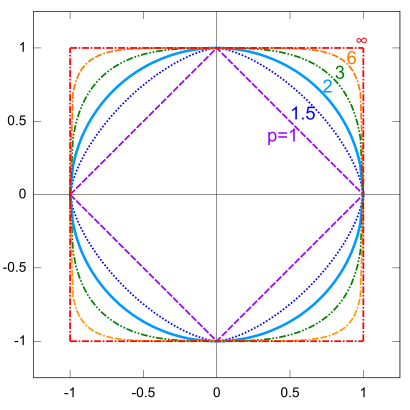
\includegraphics[width=0.35\textwidth]{pictures/einheitsphaeren.png}
\caption{Einheitskreise verschiedener $p$-Normen im $\R^2$ \cite{Einheitsphären}}
\end{figure}
\begin{sa}
\label{jede_norm_eq}
(vgl. Ref. \cite{Clason}, S.27) Ist $E$ ein endlichdimensionaler Vektorraum, so sind alle Normen auf $E$ äquivalent.
\end{sa}
\begin{bem}
Auf einen Beweis wird hier bewusst verzichtet, da auf diesem Thema nicht der Schwerpunkt dieser Arbeit liegt. Dennoch ist dieser Satz für uns sehr wichtig.
\end{bem}
\begin{dfi}
Sei $(X, {\|\cdot\|})$ ein normierter Raum und $A \subset X$.
Dann ist mit 
\begin{align*}
d(x, y) = \|x - y\| \enspace \text{für} \: x, y \in X
\end{align*}
eine Metrik auf $A$ gegeben. Man nennt sie die von der Norm $\|\cdot\|$ induzierte Metrik.
\end{dfi}
\begin{bew}
Im Folgenden weisen wir die Metrikaxiome nach und verifizieren diese Aussage:
\begin{enumerate}[label=(\roman*)]
\item Nichtdegeneriertheit: $d(x, y) = 0 \Longleftrightarrow \|x - y\| = 0 \Longleftrightarrow x - y = 0 \Longleftrightarrow x=y$
\item Symmetrie: $d(x, y) = \|x - y\| = \|(-1)(x - y)\| = |-1|\|x - y\| = d(x, y)$
\item Dreiecksungleichung:\\ $d(x, z) =\|x - z\| = \|x - y + y - z\| \leq \|x - y\| + \|y - z\| = d(x, y) + d(y, z)$
\end{enumerate}
\end{bew}
\begin{bem}
Jede Norm auf $X$ induziert also eine Metrik und zu jedem normierten Raum gehört stets ein kanonischer metrischer Raum. Im Gegensatz dazu, ist nicht jeder metrische Raum auch ein normierter Raum. Es gibt Metriken, welche die Axiome einer Norm nicht erfüllen.
\end{bem}
\begin{bew}
Ein Beispiel dafür ist die diskrete Metrik, welche das Normaxiom (ii) nicht erfüllt: 
Sei $\|x\| = d(x,0)$ und sei $x \neq 0$, so ist $\|2x\| = d(2x,0) = 1 \neq 2 = 2d(x,0) = |2|\|x\|$
\end{bew}
\noindent Zu diesem Unterkapitel möchte ich abschließend darauf hinweisen, dass wir uns konkret für normierte Räume interessieren. Viele Aussagen jedoch auch allgemeiner auf metrischen Räumen gelten. Auf diese Eigenschaft wollen wir nicht verzichten. Im Folgenden werden also einige Definitionen und Sätze über metrische Räume beschrieben.
\newpage

%%%%%%%%%%%%%%%%%%%%%%%%%%%%%%%%%%%%%%%%%%%%%%%%%%%%%%%%%%%%%%%%%%
%Banachräume
%%%%%%%%%%%%%%%%%%%%%%%%%%%%%%%%%%%%%%%%%%%%%%%%%%%%%%%%%%%%%%%%%%
\section{Banachräume}
%%%%%%%%%%%%%%%%%%%%%%%%%%%%%%%%%
%Konvergenz in normierten Räumen
%%%%%%%%%%%%%%%%%%%%%%%%%%%%%%%%%
\subsection{Konvergenz in normierten Räumen}

In der Analysis spielt die Konvergenz und auch Konvergenzprobleme eine große Rolle. Immer, wenn man sich mit Normen beschäftigt, muss man genau diese Konvergenzprobleme berücksichtigen. Deshalb möchte ich mit der Konvergenz in normierten Räumen in das Thema Banachräume einleiten. Im folgenden sei $(X,\|\cdot\|)$ ein normierter Vektorraum.
\begin{dfi}
\label{konv}
Sie ${(x_k)}_{k \in \N} = (x_1, x_2, x_3, . . .)$ eine Folge aus Elementen $x_k \in X$ des Vektorraums, dann \textit{konvergiert} diese gegen $x \in X$, wenn gilt:
\begin{align*}
& \|x - x_k\| \rightarrow 0 \enspace \text{für} \enspace k \rightarrow \infty
\end{align*}
\end{dfi}
\begin{bem}
Man schreibt dann $x_k \rightarrow x$ für $k \rightarrow \infty$ oder $\lim\limits_{n \to \infty}{x_k} = x$.
\end{bem}
Eine zu Definition  \hyperref[konv]{\ref*{konv}} äquivalente Schreibweise ist die sogenannte Epsilon-Schreibweise der Konvergenz. Sie ist etwas mathematischer über Quantoren definiert, aber besagt im Kern genau das selbe.
\begin{dfi}
\label{konv_eps}
 Die Folge ${(x_k)}_{k \in \N}$ konvergiert gegen $x \in X$, wenn gilt:
\begin{align*}
& \forall \epsilon > 0 \enspace \exists N \in \N : \|x - x_k\| \leq \epsilon \enspace \text{für alle} \enspace k \geq N
\end{align*}
\end{dfi}
\begin{bem}
Genau dann, wenn diese Bedingung gilt, ist also $x \in X$ der Grenzwert der Folge ${(x_k)}_{k \in \N}$. Besitzt die Folge hingegen keinen Grenzwert, so nennt man sie auch \textit{divergent}. Desweiteren ist eine \textit{Nullfolge} eine konvergente Folge mit dem Grenzwert 0.
\end{bem}
\begin{lem}
\label{eindeutigkeit}
Jede konvergente Folge in $X$ besitzt nur einen einzigen Grenzwert.
\end{lem}
\begin{bew}
Wir nehmen an ${(x_k)}_{k \in \N}$ sei eine Folge mit zwei verschiedenen Grenzwerten $x, y$. Dann gilt $\|x - y\| > 0$, da $x \neq y$. Sei nun $\epsilon = \frac{1}{3}\|x - y\|$, dann gilt mit Definition \hyperref[konv_eps]{\ref*{konv_eps}}:
\begin{align*}
\exists N_1 \in \N : \|x - x_k\| \leq \frac{1}{3}\|x - y\| & \enspace \text{für alle} \enspace k \geq N_1\\
\exists N_2 \in \N : \|y - x_k\| \leq \frac{1}{3}\|x - y\| & \enspace \text{für alle} \enspace k \geq N_2
\end{align*}
Damit gilt für alle Folgenglieder $x_k$ mit $k \geq \max\{N_1, N_2\}$, dass sowohl $\|x - x_k\| \leq \frac{1}{3}\|x - y\|$ als auch $\|y - x_k\| \leq \frac{1}{3}\|x - y\|$ ist. In diesem Fall wäre also 
\begin{align*}
\|x - y\| &= \|x + (-x_k + x_k) - y\|\\
&= \|(x - x_k) + (x_k - y)\| \overset{\Delta\text{-Ungl.}}\leq  \|x - x_k\| + \|x_k -y\|\\
&\leq \frac{1}{3}\|x - y\| + \frac{1}{3}\|x - y\| = \frac{2}{3}\|x - y\|.
\end{align*}
Da nach Annahme $x \neq y$ ist und somit gilt $\|x - y\| > 0$, lassen sich beide Seiten durch $\|x - y\|$ dividieren. Damit erhalten wir einen Widerspruch: $1 \leq \frac{2}{3}$.
\end{bew}
\begin{bem}
Der Grenzwert einer jeden Folge ist also eindeutig. Dieser Satz macht Ausdrücke wie $\lim_{k \to \infty}{x_k}$ erst sinnvoll. Angenommen es gäbe Folgen mit mehr als einem Grenzwert, dann könnte man dem Ausdruck $\lim_{k \to \infty}{x_k}$ keine eindeutige Zahl zuordnen.
\end{bem}
\begin{lem}
Jede konvergente Folge in $X$ ist beschränkt.
\end{lem}
\begin{bew}
Sei ${(x_k)}_{k \in \N}$ eine konvergente Folge mit Grenzwert $x$. Dann gilt mit \hyperref[konv_eps]{\ref*{konv_eps}}:
\begin{align*}
\forall \epsilon > 0 \enspace \exists N \in \N : \|x - x_k\| \leq \epsilon \enspace \text{für alle} \enspace k \geq N
\end{align*}
Daraus folgt:
\begin{align*}
\|x_k\| = \|x_k - x + x\| \overset{\Delta\text{-Ungl.}}\leq \|x_k - x\| + \|x\| \leq \epsilon + \|x\| \enspace \text{für alle} \enspace k \geq N
\end{align*}
\begin{align*}
\|x_k\| \leq \max\{\|x_1\|, \|x_2\|, ..., \|x_{N-1}\|, \epsilon + \|x\|\} \enspace \text{für alle} \enspace k \in N
\end{align*}
\end{bew}
\begin{dfi}
(vgl. Ref. \cite{Clason}, S.6) Sei ${(x_n)}_{n \in \N}$ eine Folge in X.
\begin{enumerate}[label=(\roman*)]
\item Ist ${(n_k)}_{k \in \N} \subset \N$ eine streng monoton wachsende Folge mit $n_1 < n_2 < n_3 < ...$ dann ist ${(x_{n_k})}_{k \in \N}$ eine \textit{Teilfolge} von ${(x_n)}_{n \in \N}$.
\item Hat ${(x_n)}_{n \in \N}$ eine konvergente Teilfolge mit Grenzwert $x \in X$, so heißt $x$ \textit{Häufungspunkt} von ${(x_n)}_{n \in \N}$.
\end{enumerate}
\end{dfi}
Wollen wir also jetzt herausfinden, ob eine Folge konvergiert, dann können wir dazu Definition \hyperref[konv]{\ref*{konv}} oder Definition \hyperref[konv_eps]{\ref*{konv_eps}} nutzen. Doch haben wir nur die Folge ${(x_k)}_{k \in \N}$ gegeben und wissen deren Grenzwert $x \in X$ nicht, so lassen sich diese Definitionen nicht anwenden. Damit uns diese Definitionen also von Nutzen sind, müssten wir in der Lage sein, den Grenzwert zu erraten. In manchen Fällen ist das auch möglich. Wenn man sich jedoch mit abstrakten normierten Räumen beschäftigt, kann dies nicht immer ganz trivial sein. Im Folgenden werden wir nun sehen, dass man dieses Problem Dank des mächtigen Konzepts der Cauchy-Folge umgehen kann.
\begin{dfi}
\label{konv_cau}
Eine Folge ${(x_k)}_{k \in \N}$ in $X$ ist eine \textit{Cauchy-Folge}, wenn gilt:
\begin{align*}
& \forall \epsilon > 0 \enspace \exists N \in \N : \|x_k - x_l\| \leq \epsilon \enspace \text{für alle} \enspace k,l \geq N
\end{align*}
\end{dfi}
\begin{bem}
Anders wie in Definition \hyperref[konv]{\ref*{konv}} oder Definition \hyperref[konv_eps]{\ref*{konv_eps}} wird hier nicht mehr der Abstand zwischen Grenzwert und Folgeglied betrachtet, sondern die Abstände zwischen Folgegliedern untereinander.
\end{bem}
\begin{sa}
\label{konv_ist_cauchy}
Jede konvergente Folge in $X$ ist eine Cauchy-Folge.
\end{sa}
\begin{bew}
Sei ${(x_k)}_{k \in \N}$ eine konvergente Folge mit Grenzwert x. Sei $\epsilon > 0$ dann gilt mit \hyperref[konv_eps]{\ref*{konv_eps}}:
\begin{align*}
\exists N \in \N : 
\begin{cases}
\|x - x_k\| \leq \frac{\epsilon}{2} & \enspace \text{für alle} \enspace k \geq N\\
\|x - x_l\| \leq \frac{\epsilon}{2} &\enspace \text{für alle} \enspace l \geq N
\end{cases}
\end{align*}
Sein nun $k, l \geq N$ beliebig, dann folgt:
\begin{align*}
\|x_k - x_l\| = \|(x_k - x) + (x - x_l)\| \overset{\Delta\text{-Ungl.}}\leq \underbrace{\|x_k - x\|}_{\leq \frac{\epsilon}{2}} + \underbrace{\|x - x_l\|}_{\leq \frac{\epsilon}{2}} \leq \epsilon 
\end{align*}
\end{bew}
Auch mit Satz \hyperref[konv_ist_cauchy]{\ref*{konv_ist_cauchy}} bleibt unser Problem immer noch bestehen. Würde jedoch auch die Umkehrung dieses Satzes gelten, dann könnten wir von einer Cauchy-Folge auf Konvergenz schließen und müssten nicht mehr den Grenzwert kennen oder vermuten. Tatsächlich gilt auch in sehr vielen Räumen diese Umkehrung, also: Jede Cauchy-Folge ist konvergent.
\newpage

%%%%%%%%%%%%%%%%%%%%%%%%%%%%%%%%%
%Vollständigkeit
%%%%%%%%%%%%%%%%%%%%%%%%%%%%%%%%%
\subsection{Vollständigkeit}

In diesem Unterkapitel werden wird sehen, dass die Vollständigkeit weitreichende Folgen hat und es uns ermöglicht, den Begriff Banachraum einzuführen.
\begin{dfi}
(vgl. Ref. \cite{Werner}, S.472) Ein Raum heißt \textit{vollständig}, wenn in ihm jede Cauchy-Folge konvergiert.
\end{dfi}
\begin{bsp}
Wählt man die Menge der rationalen Zahlen $\Q$ und versieht diese mit der mit der Betragsnorm $|\cdot|$ (induziert mit $d(x,y) = |x - y|$ die Betragsmetrik), so ist der Raum $(\Q, |\cdot|)$ \textit{nicht} vollständig. Definiert man nämlich die rekursive Folge ${(x_k)_{k \in \N}}$ (Iterationsgleichung des Heron-Verfahrens) mit
\begin{align*}
& x_0 := 1 \: \text{und} \: x_{k+1} := {1 \over 2}\left(x_k + {2 \over x_k}\right)
\end{align*}
sind offensichtlich alle Folgenglieder rational. Wir wollen nun zeigen, dass die Folge eine Cauchy-Folge ist und in $\R$ gegen die Zahl $\sqrt{2}$ konvergiert.
\\Wir zeigen zunächst, dass ${({x_k}^2)}_{k \in \N}$ konvergent ist.
\begin{itemize}
\item Untere Schranke (für $n\geq 1$):
\begin{align*}
&{x_k}^2 -2 = \left(\frac{1}{2}\left(x_{k -1} + \frac{2}{x_{k-1}}\right)\right)^2 - 4\cdot \frac{1}{2} \cdot x_{k-1} \cdot \frac{1}{x_{k-1} } = \left(\frac{1}{2}\left(x_{k-1} - \frac{2}{x_{k-1}}\right)\right)^2 \geq 0 \\
&\Rightarrow {x_k}^2 \geq 2 \: \text{für} \: n \geq 1
\end{align*}
\item Obere Schranke: ${x_k}^2 \leq 2 + \frac{1}{2^k} $\\\\
\textit{Beweis durch vollständige Induktion:}
\begin{itemize}
\item $k = 0: {x_0}^2 = 1^2 = 1 \leq 2 + \frac{1}{2^0} = 3$
\item Induktionsvoraussetzung : ${x_k}^2 \leq 2 + \frac{1}{2^k}$
\item $k \rightarrow k + 1$: 
\begin{align*}
{x_{k+1}}^2 &= {\left(\frac{1}{2}(x_k + \frac{2}{x_k})\right)}^2 = \frac{1}{4} \left({x_k}^2 + 4 + \frac{4}{{x_k}^2}\right)\\
&\leq \frac{1}{4} ({x_k}^2 + 6), \: \text{da} \: {x_k}^2 \geq 2\\
& \leq \frac{1}{4} \left(2 + \frac{1}{2^k} + 6 \right) \:  \text{(Induktionsvoraussetzung)}\\
& = 2 + \frac{1}{2^{k+2}} \leq 2 + \frac{1}{2^{k+1}}
\end{align*}
\end{itemize}
\end{itemize}
Damit folgt dann: $\lim_{k\to\infty}{{x_k}^2} = 2$.\\\\
Da wir mit Satz \hyperref[konv_ist_cauchy]{\ref*{konv_ist_cauchy}} wissen, dass jede konvergente Folge eine Cauchy-Folge ist, ist also ${({x_k}^2)}_{k \in \N}$ eine Cauchy-Folge. Es gilt also Folgendes: 
\begin{align*}
& \forall \epsilon > 0 \enspace \exists N \in \N : |{x_k}^2 - {x_l}^2| \leq \epsilon \enspace \text{für alle} \enspace k,l \geq N
\end{align*}
Sei nun $\epsilon > 0$. Dann gilt:
\begin{gather*}
|{x_k} - {x_l}| \leq 2 |{x_k} - {x_l}|\\
\leq (x_k + x_l)\cdot|{x_k} - {x_l}|, \text{denn} \: x_k, x_l \geq 1\\
= |(x_k + x_l) \cdot (x_k - x_l)| = |{x_k}^2 - {x_l}^2| \leq \epsilon
\end{gather*}
für alle $k, l \in N$. Also ist auch ${(x_k)_{k \in \N}}$ selbst eine Cauchy-Folge. Wir haben gesehen, dass die Folge in $\R$ gegen $\sqrt{2}$ konvergiert. Jedoch konvergiert sie nicht in $\Q$:  Würde die Folge in $\Q$ konvergieren, so müsste wegen der Eindeutigkeit des Grenzwertes (Lemma  \hyperref[eindeutigkeit]{\ref*{eindeutigkeit}}) auch $\sqrt{2} \in \Q$ gelten. Das ist aber offensichtlich \textit{nicht} der Fall! (vgl. Ref. \cite{biel})
\end{bsp}
\begin{sa}
Jeder metrische Raum $(X,d)$ kann vervollständigt werden. Es gibt einen vollständigen metrischen Raum $(\hat{X},\hat{d})$ mit einer Isometrie $\varphi: X \rightarrow \hat{X}$, sodass $\varphi(X)$ dicht in $\hat{X}$ liegt. Der Raum $(\hat{X},\hat{d})$ heißt \textit{Vervollständigung} von $(X,d)$.
\end{sa}
\begin{bem}
Im Fall der rationalen Zahlen $\Q$ erhält man durch Vervollständigung den Raum der reellen Zahlen $\R$.
Alle Vervollständigungen von $(X,d)$ sind \textit{isometisch isomorph}. Auf einen Beweis wird verzichtet.
\end{bem}
Vollständigkeit lässt uns also von Cauchy-Folgen auf Konvergenz schließen. Ist ein normierter Vektorraum vollständig, so kommen wir zu der wichtigsten Definition in diesem Kapitel.
\begin{dfi}
(vgl. Ref. \cite{Alt}, S.28) Ein normierter Vektorraum $X$ heißt \textit{Banachraum}, wenn er vollständig (bezüglich der induzierten Metrik) ist.
\end{dfi}
\begin{bem}
Tatsächlich sind sogar die meisten Räume, mit denen man sich in der angewandten Mathematik beschäftigt, Banachräume. (z.B $\R, \R^n, \C, \C^n$)
\end{bem}
Ich weise noch einmal darauf hin, dass wir uns auf die Fälle $\K = \R$ oder $\K = \C$ beschränken.
\begin{sa}
Der Raum $(\K^n, \|\cdot\|_2)$ ist ein Banachraum.
\end{sa}
\begin{bew}
Sei ${(x_k)_{k \in \N}}$ eine Cauchy-Folge in $(\K^n, \|\cdot\|_2)$. Dann gilt für alle $j = 1, ..., n$ und für jedes $\epsilon > 0$:
\begin{align*}
|x_{k,j} - x_{l,j}| \leq \|x_k - x_l\|_2 \leq \epsilon \enspace \text{für alle} \: k,l \geq N
\end{align*}
Somit ist jede Komponentenfolge ${(x_{k,j})_{k \in \N}}$ eine Cauchy-Folge in $\K$. Da nun aber $\K$ vollständig ist, gibt es damit auch dessen Grenzwert $\lim\limits_{k \to \infty}{x_{k,j}} = x_j$ und somit findet man
\begin{align*}
\lim_{k \to \infty}{x_k} = \lim_{k \to \infty} \left(\begin{array}{c} a_{k,1} \\ a_{k,2} \\ \vdots \\ a_{k,n} \end{array}\right) = \left(\begin{array}{c} \lim\limits_{k \to \infty}{a_{k,1}} \\ \lim\limits_{k \to \infty}{a_{k,2}} \\ \vdots \\ \lim\limits_{k \to \infty}{a_{k,n}} \end{array}\right) = \left(\begin{array}{c} x_1 \\ x_2 \\ \vdots \\ x_n \end{array}\right) = x \in \K^n
\end{align*}
\end{bew}
\begin{bem}
Die Vollständigkeit von $\K^n$ wird auf die Vollständigkeit von $\K$ zurückgeführt. Die Vollständigkeit von $\K$ ist jedoch ein Postulat, d.h. $\K$ ist gemäß seiner Definition vollständig.
\end{bem}
Ist $E$ ein endlichdimensionaler Vektorraum, dann gilt insbesondere, dass $(E, \|\cdot\|_2)$ vollständig ist, da $(\K^n, \|\cdot\|_2)$ vollständig ist.
Mit Satz \hyperref[jede_norm_eq]{\ref*{jede_norm_eq}} wissen wir, dass alle Normen auf endlichdimensionalen Vektorräumen äquivalent sind. Da nun die Vollständigkeit beim Übergang zu äquivalenten Normen erhalten bleibt und $(E, \|\cdot\|_2)$ vollständig ist, können wir sogar eine noch allgemeinere Folgerung treffen. 
\begin{fol}
\label{vollundendlich}
(vgl. Ref. \cite{Clason}, S.28) Alle endlichdimensionalen normierten Vektorräume sind vollständig und somit Banachräume.
\end{fol}
\begin{bem}
Hingegen zu endlichdimensionalen normierten Vektorräumen, müssen unendlichdimensionale normierten Räumen nicht immer vollständig sein.
\end{bem}
\begin{fol}
(vgl. Ref. \cite{Clason}, S.24) Sind ${\|\cdot\|}_1$ und ${\|\cdot\|}_2$ äquivalente Normen auf dem Vektorraum $X$ , dann ist $(X , {\|\cdot\|}_1)$ ein Banachraum genau dann, wenn $(X , {\|\cdot\|}_2)$ ein Banachraum ist.
\end{fol}
\newpage

%%%%%%%%%%%%%%%%%%%%%%%%%%%%%%%%%
%Vollständigkeit der Folgen- und Funktionenräume
%%%%%%%%%%%%%%%%%%%%%%%%%%%%%%%%%
\subsection{Vollständigkeit der Folgen- und Funktionenräume}
Wir betrachten nun die einfachsten Beispiele für unendlichdimensionale normierte Räume. Dazu wollen wir uns zunächst die Funktionenräume und anschließend die Folgenräume genauer ansehen. Da es in der Funktionalanalysis eine Vielzahl an solchen Räumen gibt, betrachten wir in diesem Unterkapitel jeweils einen Funktionenraum und einen Folgenraum etwas ausführlicher und zeigen dann auch, dass diese vollständig sind.
\begin{dfi}
Sei $D$ eine nichtleere Menge und $X$ ein Vektorraum über $\K$, dann bezeichnet $Abb(D,X)$ die Menge aller Funktionen von $D$ nach $X$:
\begin{align*}
Abb(D,X) := \{f \: | \: f : D \rightarrow X\}
\end{align*}
\end{dfi}
\begin{bem}
Da wir den Funktionenraum auf einem Vektorraum definieren, spricht man hier auch von einem linearen Funktionenraum. Die Menge ist also abgeschlossen bezüglich der Addition und Skalarmultiplikation:
\begin{itemize}
\item[(i)]  $+ : Abb(D,X) \times Abb(D,X) \rightarrow Abb(D,X), (f + g)(x) = f(x) + g(x)$\\
\item[(ii)]  $\cdot :  \K \times Abb(D,X) \rightarrow Abb(D,X), (\lambda f)g(x) = \lambda f(x)$
\end{itemize}
\end{bem}
In der Funktionalanalysis gibt es eine Vielzahl an Funktionenräumen, die untersucht werden. Beispiele hierfür wären Räume stetiger und differenzierbarer Funktionen,  Lebesgue- und Bocher-Räume oder auch Sobolev-Räume. Wir wollen uns hier aber auf den Raum der stetigen Funktionen beschränken, da dies sonst den Rahmen der Arbeit übertreffen würde.
\begin{dfi}
Raum der stetigen Funktionen auf dem Intervall $[a,b] \subset \K$:
\begin{align*}
C([a,b], X) := \left\{ f : [a,b] \rightarrow X \: | \: f \: \text{ist stetig} \right\}
\end{align*}
Falls $X = \R$ wird es auch oft weggelassen und wir schreiben dann kurz dafür $C[a,b]$.
\end{dfi}
\begin{bem}
Räume von stetigen Funktionen können auch für allgemeine topologische Räume als Urbild (und Definitionsbereich) definiert werden.
\end{bem}
\begin{dfi}
Sei $D$ eine nichtleere Menge und sei $f : D \rightarrow \K$ eine beschränkte Funktion, dann bezeichnet man Folgendes als die \textit{Supremumsnorm} von $f$:
\begin{align*}
\|f\|_\infty = \sup_{x \in D}{|f(x)|}
\end{align*}
\end{dfi}
Wenn wir uns an die Analysis zurückerinnern, dann heißt eine Funktion beschränkt, wenn es einen Wert gibt, der größer oder kleiner als alle anderen Funktionswerte ist. Da wir uns im Raum der stetigen Funktionen auf einem kompakten Intervall bewegen, gilt sogar folgendes Lemma vom Minimum und Maximum aus der Analysis.
\begin{lem}
\label{besch}
Jede auf einem kompakten Intervall $[a,b] \subset \R$ definierte Funktion ist dort beschränkt und nimmt dort ein Minimum und ein Maximum an.
\end{lem}
\begin{bem}
Da dieses Lemma bereits bekannt sein sollte, wird auf einen Beweis verzichtet.
\end{bem}
\begin{sa}
Der Raum $(C[a,b], \|\cdot\|_\infty)$ ist vollständig.
\end{sa}
\begin{bew}
Sei ${(f_k)}_{k \in \N}$ eine Cauchy-Folge in $(C[a,b], \|\cdot\|_\infty)$, dann gilt nach Definition \hyperref[konv_cau]{\ref*{konv_cau}}:
\begin{align*}
& \forall \epsilon > 0 \enspace \exists N \in \N : \|f_k - f_l\|_\infty \leq \epsilon \enspace \text{für alle} \enspace k,l \geq N
\end{align*}
Es muss nun gezeigt werden, dass eine stetige Grenzfunktion $f \in C[a,b]$ existiert, sodass $\|f - f_l\|_\infty \rightarrow 0$ für $l \rightarrow \infty$.
Hierzu benutzen wir die Beziehung zwischen den Funktionswerten und der Supremumsnorm:
\begin{align*}
|f_k(x) - f_l(x)| \leq \max_{x \in [a,b]}{|f_k(x) - f_l(x)|} = \|f_k - f_l\|_\infty
\end{align*}
Für festes $x \in [a,b]$ ist $f_k(x)$ eine Cauchy-Folge im Raum der reellen Zahlen:
\begin{align*}
& \forall \epsilon > 0 \enspace \exists N \in \N : |f_k(x) - f_l(x)| \leq \epsilon \enspace \text{für alle} \enspace k,l \geq N
\end{align*}
Mit Folgerung \hyperref[vollundendlich]{\ref*{vollundendlich}} wissen wir, dass alle endlichdimensionalen normierten Vektorräume Banachräume sind. Wie bereits erwähnt, ist damit insbesondere $\R$ ein Banachraum. Damit folgt die Existenz der Grenzfunktion $f(x) = \lim_{k \to \infty}{f_k(x)}$ und es gilt:
\begin{align*}
& \forall \epsilon > 0 \enspace \exists N \in \N : |f(x) - f_l(x)| \leq \epsilon \enspace \text{für alle} \enspace l \geq N
\end{align*}
Analog, wie zuvor, können wir wieder die Beziehung zwischen Funktionswerten und Supremumsnorm nutzen:
\begin{align*}
 |f(x) - f_l(x)| \leq \max_{x \in [a,b]}{|f(x) - f_l(x)|} = \|f - f_l(x)\|_\infty
\end{align*}
Wir erhalten also folgenden Ausdruck:
\begin{align*}
& \forall \epsilon > 0 \enspace \exists N \in \N : \|f - f_l(x)\|_\infty \leq \epsilon \enspace \text{für alle} \enspace l \geq N
\end{align*}
Somit ist gezeigt, dass $(C[a,b], \|\cdot\|_\infty)$ vollständig ist.
\end{bew}
\begin{bem}
Da in diesem Raum auch alle Normbedingungen erfüllt sind, ist er sogar ein Banachraum. In diesem Beweis wurde darauf verzichtet, zu zeigen, dass die Grenzfunktion auch eine stetige Funktion ist. Streng genommen müsste man das aber noch zeigen.
\end{bem}
\begin{dfi}
(vgl. Ref. \cite{Clason}, S.29) Die Menge $\omega$ bezeichnet die Menge aller Folgen über $\K$:
\begin{align*}
\omega := \{{(x_k)}_{k \in \N} : x_k \in \K \: \text{für alle} \: k \in \N\}
\end{align*}
Man nennt $\omega$ dann auch den Folgenraum über $\K$.
\end{dfi}
\begin{bem}
Man vergewissert sich leicht, dass diese Menge alle acht Vektorraumaxiome aus Definition \hyperref[vektorraum]{\ref*{vektorraum}} erfüllt und somit Folgendes gilt. (Auf den Beweis wird verzichtet.)
\end{bem}
\begin{sa}
\label{folgenraum-vektorraum}
Der Folgenraum ist ein $\K$-Vektorraum.
\end{sa}
Im Folgenden sehen wir uns eine Teilmenge von $\omega$ etwas genauer an. 
\begin{dfi}
(vgl. Ref. \cite{Clason}, S.29) Raum der beschränkten Folgen:
\begin{align*}
 \ell^\infty(\K) := &\left\{x \in \omega \: \big\vert \: x = {(x_k)}_{k \in \N} \: \text{ist beschränkt} \Leftrightarrow \sup_{k \in \N}{|x_k|} < \infty \right\}
\end{align*}
\end{dfi}
\begin{bem}
Es lässt sich leicht zeigen, dass diese Teilmenge abgeschlossen bezüglich der komponentenweisen Addition und Skalarmultiplikation ist und somit einen Unterraum des Folgenraums bildet.
\end{bem}
\begin{bew}
Im Folgenden wollen wir also die drei Unterraumkriterien aus Definition \hyperref[unterraum]{\ref*{unterraum}} nachweisen.
\begin{enumerate}[label=(\roman*)]
\item Das Nullelement von $\omega$ ist die Folge, die konstant 0 ist. Diese ist natürlich beschränkt (z.B. durch 1) und liegt somit in $\ell^\infty$. Damit ist $\ell^\infty \neq \emptyset$.
\item Sein $x = {(x_k)}_{k \in \N}, y = {(y_k)}_{k \in \N} \in \ell^\infty$. Dann folgt mit der Dreiecksungleichung:
\begin{align*}
\sup_{k \in \N}{|{x_k} + {y_k}|} \overset{\Delta\text{-Ungl.}}\leq  \sup_{k \in \N}{(|{x_k}| + |{y_k}|)} \leq \underbrace{\sup_{k \in \N}{|{x_k}|}}_{< \infty} + \underbrace{\sup_{k \in \N}{|{x_k}|}}_{< \infty} < \infty
\end{align*}
Somit ist $x + y \in \ell^\infty$ und damit abgeschlossen bezüglich der Addition.
\item Sei $x = {(x_k)}_{k \in \N} \in \ell^\infty$ und  $\lambda \in \K$. Mit $|\lambda x_k| = |\lambda| |x_k|$ für alle $k \in \N$ folgt dann:
\begin{align*}
\sup_{k \in \N}{|\lambda {x_k}|} = \sup_{k \in \N}{(|\lambda| |{x_k}|)} = |\lambda| \underbrace{\sup_{k \in \N}{|{x_k}|}}_{< \infty} < \infty
\end{align*}
Somit ist $|\lambda| x \in \ell^\infty$ und damit abgeschlossen unter der Skalarmultiplikation.
\end{enumerate}
\end{bew}
\noindent Wir versehen den Raum der beschränkten Folgen $\ell^\infty$ nun mit der  Supremumsnorm:
\begin{align*}
\|x\|_\infty = \sup_{k \in \N}{|x_k|} \quad \text{für} \: x = {(x_k)}_{k \in \N}
\end{align*}
\begin{sa}
(vgl. Ref. \cite{Clason}, S.30) Der Raum $(\ell^\infty(\K), \|\cdot\|_\infty)$ ist vollständig.
\end{sa}
\begin{bew}
Sei ${(x_k)}_{k \in \N}$ eine Cauchy-Folge in $(\ell^\infty(\K), \|\cdot\|_\infty)$, dann gilt nach Definition \hyperref[konv_cau]{\ref*{konv_cau}}:
\begin{align*}
& \forall \epsilon > 0 \enspace \exists N \in \N : \|x_k - x_l\|_\infty \leq \epsilon \enspace \text{für alle} \enspace k,l \geq N
\end{align*}
Um die Vollständigkeit dieses Raums zu beweisen, betrachten wir Folgen von Folgen und schreiben dafür $x = {(x(n))}_{n \in \N} \in \omega$.  Es muss nun gezeigt werden, dass ein Grenzwert $x \in \ell^\infty$ existiert und $\|x - x_l\|_\infty \rightarrow 0$ für $l \rightarrow \infty$ gilt. Wir benutzen folgende Beziehung:
\begin{align*}
|x_k(n) - x_l(n)| \leq \|x_k - x_l\|_\infty \enspace \text{für alle} \enspace  n \in \N
\end{align*}
Für $n \in \N$ ist $x_k(n)$ eine Cauchy-Folge im Raum den reellen Zahlen:
\begin{align*}
& \forall \epsilon > 0 \enspace \exists N \in \N : |x_k(n) - x_l(n)| \leq \epsilon \enspace \text{für alle} \enspace k,l \geq N, n \in \N
\end{align*}
Auf Grund der Vollständigkeit von $\R$ existiert ein Grenzwert $x(n) = \lim\limits_{k \to \infty}{x_k(n)}$ in $\R$ und es existiert weiterhin ein $L(n)$, sodass gilt:
\begin{align*}
& \forall \epsilon > 0 \enspace \exists N \in \N : |x(n) - x_L(n)| \leq \epsilon \enspace \text{für alle} \enspace L(n) \geq N, n \in \N
\end{align*}
Für alle $k \geq N$ gilt dann:
\begin{align*}
& |x_k(n) - x(n)| \leq |x_k(n) - x_{L(n)}(n)| + |x_{L(n)}(n) - x(n)| \leq 2\epsilon  
\end{align*}
Damit folgt, dass der Grenzwert $x \in \ell^\infty$ beschränkt ist:
\begin{align*}
& |x(n)| \leq |x_N(n)| + | x(n) - x_N(n)| \leq \|x_N\|_\infty + 2\epsilon < \infty
\end{align*}
Desweiteren folgt durch Supremum über alle $n \in N$ 
\begin{align*}
& \|x_k - x\|_\infty \leq 2\epsilon 
\end{align*}
Damit ist gezeigt, dass $(\ell^\infty(\K), \|\cdot\|_\infty)$ vollständig ist. (vgl. Ref. \cite{Clason}, S.30)
\end{bew}
\begin{bem}
Auch hier lassen sich alle Normbedingungen nachweisen. $(\ell^\infty(\K), \|\cdot\|_\infty)$ ist also sogar ein Banachraum.\\ \\ Es ist leicht zu sehen, dass eine Folge in $\K^n$ genau dann konvergiert, wenn jede Komponente konvergiert. Dies ist in $\ell^\infty$ nicht der Fall, wie man an der Folge $x_k := (0, 0, ..., 0, 1, 1, ...)$ (zuerst $ k$ Nullen, dann nur noch Einsen) sieht. Diese Folge konvergiert komponentenweise gegen den Nullvektor $0 = (0, 0, 0, . . .)$, jedoch $ \|x_k - 0\|_\infty = 1 \nrightarrow 0$.
\end{bem}
\newpage
%%%%%%%%%%%%%%%%%%%%%%%%%%%%%%%%%
%Abgeschlossenheit
%%%%%%%%%%%%%%%%%%%%%%%%%%%%%%%%%
\subsection{Abgeschlossenheit}

Der Begriff der abgeschlossenen Menge lässt sich auf verschiedenen Abstraktionsstufen definieren. Im Folgenden wird hier aber nur der metrische Raum betrachtet und nicht etwa der noch allgemeinere topologische Raum. Es sei also $(X, d)$ ein metrischer Raum.
\begin{dfi}
(vgl. Ref. \cite{Clason}, S.4) Wir definieren für $x \in X$ und $r >0$
\begin{itemize}
\item[(i)] die \textit{offene Kugel} $U_r (x) := \{y \in X : d(x, y) < r \}$ 
\item[(ii)] die \textit{abgeschlossene Kugel} $B_r (x) := \{y \in X : d(x, y) \leq r \}$ 
\end{itemize}
um den Punkt $x$ mit Radius $r$.
\end{dfi}
\begin{bem}
Der Begriff einer Kugel spielt in vielen Teilgebieten der Mathematik eine wesentliche Rolle in Definitionen oder auch Beweisen. Auch wir werden diesen Begriff in den folgenden Unterkapiteln dringend benötigen. Es lässt sich damit z.B. auch der folgende Begriff einer offenen Teilmenge definieren.
\end{bem}
\begin{dfi}
(vgl. Ref. \cite{Clason}, S.4) Eine Menge $O \subset X$ heißt offen, wenn gilt:
\begin{align*}
 \forall x \in O \enspace \exists \epsilon > 0 : U_\epsilon(x) \subset O
\end{align*}
\end{dfi}
Eine dazu äquivalente Definition (über innere Punkte) ist Folgende.
\begin{dfi}
$O \subset X$ heißt \textit{offen}, wenn jedes $x \in O$ ein innerer Punkt von $O$ ist.
\end{dfi}
\noindent Die abgeschlossene Menge lässt sich über das offene Komplement definieren.
\begin{dfi}
(vgl. Ref. \cite{Clason}, S.4) $A \subset X$ heißt \textit{abgeschlossen}, wenn die Menge $X \setminus A$ offen ist.
\end{dfi}
\begin{bem}
Man schreibt auch kurz $A^c$ anstatt von $X \setminus A$.
\end{bem}
\begin{figure}[h]
\centering
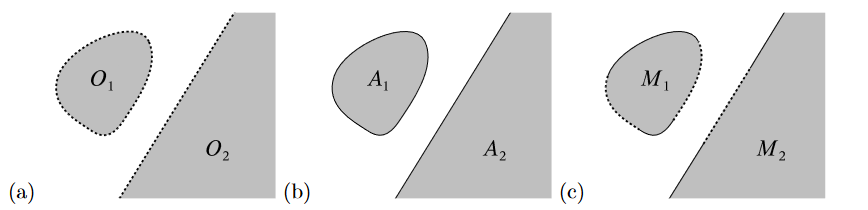
\includegraphics[width=0.80\textwidth]{pictures/offene-abgeschlossene-mengen.png}
\caption{(a) offene Teilmengen in $\R^2$. (b) abgeschlossene Teilmengen in $\R^2$. (c) Teilmengen des $\R^2$, welche weder offen noch abgeschlossen sind. \cite{OffeneAbgeschlosseneMengen}}
\end{figure}
\newpage
\begin{dfi}
\label{Umgebung}
(vgl. Ref. \cite{Clason}, S.4)  Eine Menge $U \subset X$ heißt
\begin{enumerate}[label=(\roman*)]
\item \textit{Umgebung} von $x \in U$, falls eine offene Menge $O$ mit $x \in O \subset U$ existiert;
\item \textit{Umgebung} von $A \subset U$, falls $U$ Umgebung aller $x \in A$ ist.
\end{enumerate}
\end{dfi}
\noindent Jetzt wo wir die Umgebungen definiert haben, können wir die Gelegenheit nutzen, um den Konvergenzbegriff noch etwas zu erweitern. Befinden wir uns nämlich allgemeiner auf metrischen Räumen, so lässt sich die Konvergenz folgendermaßen beschreiben.
\begin{dfi}
\label{konv_metrik}
(vgl. Ref. \cite{Clason}, S.5) Eine Folge ${(x_k)}_{k \in \N} \subset X$ konvergiert in $X$ gegen den Grenzwert $x \in X$ falls eine der folgenden äquivalenten Eigenschaften gilt:
\begin{enumerate}[label=(\roman*)]
\item $\forall \epsilon > 0 \enspace \exists N \in \N : d(x_k,x) \leq \epsilon \enspace \text{für alle} \enspace k \geq N$
\item Für jede Umgebung $U$ von x existiert ein $N \in \N$ mit $x_k \in U$ für alle $k \geq N$
\end{enumerate}
\end{dfi}
\begin{bem}
Wenden wir die von der Norm induzierte Metrik $d(x_k, x) = \|x - x_k\|$ auf (i) an, so erhalten wir damit Definition \hyperref[konv_eps]{\ref*{konv_eps}}. Dies zeigt, dass (i) eine Verallgemeinerung von der bereits bekannten Konvergenzdefinition in normierten Räumen ist.
\end{bem}
\begin{dfi}
(vgl. Ref. \cite{Clason}, S.5) $A \subset X$ heißt \textit{beschränkt}, falls sie einen endlichen Durchmesser besitzt:
\begin{align*}
\text{diam}(A) = \sup_{x,y \in A}{d(x,y)} < \infty
\end{align*}
\end{dfi}
\begin{bem}
Mit anderen Worten könnte man sagen, wenn wir um eine Menge eine Kugel mit endlichem Durchmesser legen können, so heißt diese beschränkt.
\end{bem}
\begin{dfi}
Für $M \subset X$ definieren wir:
\begin{itemize}
\item[(i)] das \textit{Innere} $M^\circ = M \setminus \partial M$
\item[(ii)] den \textit{Abschluss} $\bar{M} = M \cup \partial M$
\end{itemize}
\end{dfi}
\begin{figure}[h]
\centering
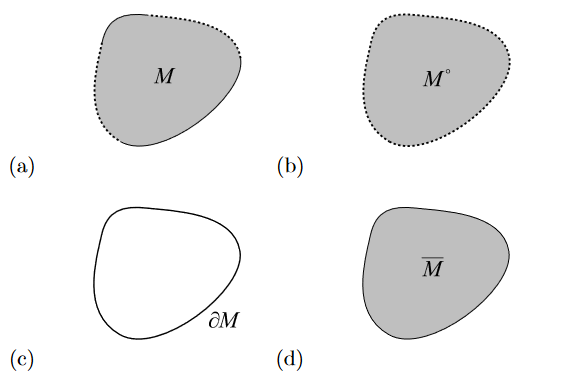
\includegraphics[width=0.50\textwidth]{pictures/innerer-abschluss.png}
\caption{(a) offene Teilmengen in $\R^2$. (b) abgeschlossene Teilmengen in $\R^2$. (c) Teilmengen des $\R^2$, welche weder offen noch abgeschlossen sind. \cite{OffeneAbgeschlosseneMengen}}
\end{figure}
\newpage
\noindent Wie anfangs erwähnt, hat die Funktionalanalysis und insbesondere das Thema Banachräume viel mit Konvergenz und Konvergenzproblemen zu tun. Deshalb ist es sinnvoll auch die Abgeschlossenheit einer Menge über den Konvergenzbegriff zu charakterisieren. Mit folgendem Satz lässt sich das problemlos durchführen.
\begin{sa}
(vgl. Ref. \cite{Forster}, S.23) Eine Teilmenge $A \subset X$ ist genau dann abgeschlossen, wenn der Grenzwert jeder konvergenten Folge in $A$ ein Element von $A$ ist.
\end{sa}
\begin{bew}
$\Rightarrow$: Sei $A$ abgeschlossen vorausgesetzt und $x_k \in A, k \in \N$, eine Folge mit $\lim_{k \to \infty}{x_k} = x$. Wir nehmen an $x \notin A$. Da A nach Voraussetzung abgeschlossen ist, ist das Komplement $X \setminus A$ offen. Somit ist $X \setminus A$ eine Umgebung von $x$. Nach Definition \hyperref[konv_metrik]{\ref*{konv_metrik}} gibt es ein $N \in \N$, sodass $x_k \in X \setminus A$ für alle $k \geq N$. Das ist aber ein Widerspruch, da $x_k \in A$ gilt.\\\\
$\Leftarrow$: Das Folgenkriterium sei erfüllt; wir wollen zeigen, dass dann $A$ abgeschlossen, d.h $X \setminus A$ offen ist. Sei $x \in X \setminus A$ ein beliebiger Punkt.\\\\
\textit{Behauptung}: Es gibt ein $\epsilon \geq 0$ mit $U_\epsilon(x) \subset X \setminus A$. Wäre dies nicht der Fall, könnten wir zu jedem $k > 0$ ein $x_k \in A$ finden mit $d(x_k,x) < 1/k$. Dann gilt aber $\lim_{k \to \infty}{x_k} = x \in A$, was im Widerspruch zu $x \in X \setminus A$ steht. Die Behauptung ist also richtig, was zeigt, dass $X \setminus A$ offen ist. (vgl. Ref. \cite{Forster}, S.23)
\end{bew}
\begin{bem}
Auf diese Weise kann man oft die Abgeschlossenheit einer Menge widerlegen.
\end{bem}
\begin{bsp}
Wir wollen zeigen, dass das Intervall $(0,1] \subset \R$ nicht abgeschlossen ist.\\
Hierzu suchen wir uns eine Folge aus, die auf dem Intervall definiert ist. Die offensichtlichste Folge wäre: $x_k = \frac{1}{k}$. Bilden wir nun den Grenzwert dieser Folge, so erhalten wir $\lim_{k \to \infty}{\frac{1}{k}} = 0$. Es gilt jedoch $0 \notin (0,1] \subset \R$ und damit ist $(0,1] \subset \R$ nicht abgeschlossen.
\end{bsp}
\begin{sa}
\label{abgeschlossenerUnterraum}
(Ref. \cite{Clason}, S.25) Sei $(X , {\|\cdot\|})$ ein Banachraum und $U \subset X$ ein Unterraum. Dann ist $(U , {\|\cdot\|})$ ein Banachraum genau dann, wenn U abgeschlossen ist.
\end{sa}
\begin{bew}
Man vergewissert sich zunächst leicht, dass $(U , {\|\cdot\|})$ ein normierter Vektorraum ist. Sei nun $U$ abgeschlossen und $(x_k)_{k \in \N} \subset U$ eine Cauchy-Folge. Da $X$ vollständig ist, konvergiert $x_k \rightarrow x \in X$ , und aus der Abgeschlossenheit von $U$ folgt $x \in U$.\newline
Sei andererseits $U$ vollständig und $(x_k)_{k \in \N} \subset U$ mit $x_k \rightarrow x \in X$ , dann ist $(x_k)_{k \in \N}$ insbesondere eine Cauchy-Folge (in $X$ und damit ebenso in $U$ ) und besitzt wegen der Vollständigkeit von $U$ einen Grenzwert $ \tilde{x}\in U$ . Da Grenzwerte eindeutig sind, muss $x =\tilde{x} \in U$ gelten. Also ist $U$ abgeschlossen.\\ 
(Ref. \cite{Clason}, S.25) 
\end{bew}
Zum Abschluss dieses Unterkapitels möchte ich noch einmal kurz darauf hinweisen, inwiefern Abgeschlossenheit und Vollständigkeit zusammenhängen bzw. sich unterscheiden. Vollständigkeit ist immer auf einem Raum selbst definiert. Abgeschlossenheit hingegen auf Teilmengen eines umfassenden Raumes. Auf der einen Seite haben wir Cauchy-Folgen, die konvergieren und auf der anderen Seite konvergente Folgen, deren Grenzwert in der Menge selbst liegt. Wir werden später noch sehen, dass diese beiden Begriffe im $\R^n$ sogar äquivalent zueinander sind, jedoch allgemein diese Äquivalenz nicht gilt.
\newpage

%%%%%%%%%%%%%%%%%%%%%%%%%%%%%%%%%
%Separabilität
%%%%%%%%%%%%%%%%%%%%%%%%%%%%%%%%%
\subsection{Separabilität}

Der Begriff separabel bezeichnet in der Topologie eine häufig benutzte Abzählbarkeitseigenschaft von topologischen Räumen. Der Begriff ist dabei von besonderer Bedeutung in der Funktionalanalysis. Man kann beispielsweise zeigen, dass es in einem separablen Hilbertraum stets abzählbare Orthonormalbasen gibt. Für normierte Räume kann die Separabilität als eine Art Größenabmessung angesehen werden.
\begin{dfi}
$M \subset X$ heißt \textit{dicht} in $X$, wenn eine der folgenden äquivalenten Aussagen zutrifft:
\begin{itemize}
\item[(i)] Zu jedem $x \in X$ und  $r > 0$ existiert ein Punkt $y \in M$: $d(x,y)<r$
\item[(ii)] Zu jedem $x \in X$ und  $r > 0$ existiert ein Punkt $y \in M$: $y \in U_r (x)$
\item[(iii)] Zu jedem $x \in X$ existiert eine Folge ${(x_n)}_{n \in \N}$ von Punkten aus M: $\lim_{n \to \infty}{x_n} = x$
\item[(iv)] Die \textit{abgeschlossene Hülle} der Menge $M$ ist der ganze Raum: $\bar{M} = X$
\end{itemize}
\end{dfi}
\begin{dfi}
$M \subset X$ heißt \textit{nirgends dicht}, wenn $M$ keinen inneren Punkt besitzt: $(\overline{M})^\circ = \emptyset$.
\end{dfi}
\begin{bem}
Die dichte Menge ist nie nirgends dicht. Um uns davon zu überzeugen, nehmen wir das Gegenteil an. Es sei $M$ eine dichte Teilmenge von $X$, die nirgends dicht ist. Da $X$ offen ist, gilt $X^\circ = X$. Da $M$ dicht in $X$ liegt, folgt $(\overline{M})^\circ = X^\circ = X = \emptyset$, was ein Widerspruch zur Annahme ist.
\end{bem}
\begin{lem}
\label{dicht}
Sei $O \subset X$ und A das Komplement von $O$, dann gilt folgende Äquivalenz:
\begin{align*}
O \: \text{ist offen und dicht} \: \Leftrightarrow A \: \text{ist abgeschlossen und nirgends dicht}
\end{align*}
\end{lem}
\begin{bew}
$\Rightarrow$: Sei $O$ offen und dicht, dann ist $A$ als Komplement einer offenen Menge abgeschlossen. Es bleibt noch zu zeigen, dass $A^\circ = \emptyset$. Da $O$ dicht in $X$ liegt gilt:
\begin{align*}
A^\circ = (\overline{A^c})^c  = (\overline{O})^c = X^c = \emptyset
\end{align*}
 Die Rückrichtung folgt analog. 
\end{bew}
\begin{dfi}
Existiert eine Menge $S \subset X$, die abzählbar und dicht in $X$ ist, so heißt diese \textit{separabel}.
\end{dfi}
\begin{bem}
Ein topologischer Raum mit abzählbarer Basis (zweites Abzählbarkeitsaxiom) ist separabel. Man erhält die abzählbare dichte Teilmenge, indem man aus jeder Menge in der Basis einen Punkt auswählt.
\end{bem}
\begin{bsp}
\quad
\begin{itemize}
\item Die Räume $\mathbb {R} ^{n}$ sind für $n\in \mathbb {N}$ separabel, da ${\mathbb {Q}}^{n}$ abzählbar ist und dicht in $\mathbb {R} ^{n}$ liegt.
\item Der Raum $c_{0}$ der Nullfolgen ist mit der Supremumsnorm separabel.
\item Der Raum der beschränkten Folgen $\ell ^{{\infty }}$ ist nicht-separabel.
\end{itemize}
\end{bsp}
\newpage

%%%%%%%%%%%%%%%%%%%%%%%%%%%%%%%%%
%Satz von Baire
%%%%%%%%%%%%%%%%%%%%%%%%%%%%%%%%%
\subsection{Satz von Baire}
Der Satz von Baire ist in verschiedenen angrenzenden Teilgebieten der Mathematik, wie der deskriptiven Mengenlehre, der Maßtheorie und vor allem der Funktionalanalysis von erheblicher Bedeutung. So lässt sich z.B. der Satz von Banach-Steinhaus, das Prinzip der gleichmäßigen Beschränktheit oder auch der Satz über die offene Abbildung, aus dem Satz von Baire ableiten.
\begin{dfi}
(vgl. Ref. \cite{Werner}, S.138) Sei $(X,d)$ ein metrischer Raum, dann gelten folgende Aussagen:
\begin{enumerate}[label=(\roman*)]
\item $M \subset X$ \textit{nirgends dicht} in $X \Leftrightarrow (\bar{M})^\circ = \emptyset$
\item $M \subset X$ \textit{von 1.Kategorie} in $X \Leftrightarrow M = \bigcup\limits_{n \in \N}{\delta_n}$, $\delta_n$ nirgends dicht
\item $M \subset X$ \textit{von 2.Kategorie} in $X \Leftrightarrow M$ ist nicht von \textit{von 1.Kategorie}
\end{enumerate}
\end{dfi}
\begin{bem}
Baires Kategorienbegriff beschreibt die Vorstellung von der Größe einer Menge im topologischem Sinn.
\end{bem}
\begin{sa}
\label{sa_baire}
$(X,d)$ sei ein vollständiger metrischer Raum. Folgende Aussagen sind äquivalent:
\begin{enumerate}[label=(\roman*)]
\item Sei ${(O_n)}_{n \in \N}$ eine offene und dichte Teilmengen $\Rightarrow \bigcap\limits_{n \in \N}{O_n}$ ist dicht
\item Sei $(A_n)_{n \in \N}$ eine abgeschlossene Teilmenge mit leerem Inneren $\Rightarrow \bigcup\limits_{n \in \N}{A_n}$ hat ein leeres Inneres
\item Jede offene nicht leere Teilmenge  ist von 2.Kategorie
\end{enumerate}
\end{sa}
\begin{bew}
(i) Setze $D = \bigcap\limits_{n \in \N}{O_n}$. Es ist zu zeigen, dass jede offene $\epsilon$-Kugel in $X$ ein Element von $D$ enthält.\\
Sei $U_\epsilon(x_0) = \{x \in X: d(x,x_0) < \epsilon\}$ eine solche Kugel. Da $O_1$ offen und dicht ist, ist $O_1 \cap U_\epsilon(x_0)$ offen und nicht leer. Es existieren also $x_1 \in O_1, \epsilon_1 > 0$ (ohne Einschränkung $\epsilon_1 < \frac{1}{2}\epsilon$) mit
\begin{align*}
U_{\epsilon_1}(x_1) \subset O_1 \cap U_\epsilon(x_0)
\end{align*}
Nach eventueller Verkleinerung von $\epsilon_1$ erhält man sogar
\begin{align*}
\overline{U_{\epsilon_1}(x_1)} \subset O_1 \cap U_\epsilon(x_0).
\end{align*}
Betrachte nun $O_2$. Auch $O_2$ ist offen und dicht, daher ist $O_2 \cap U_{\epsilon_1}(x_1)$ offen und nicht leer. Wie oben existieren $x_2 \in O_2, \epsilon_2 < \frac{1}{2}\epsilon_1$ mit
\begin{align*}
\overline{U_{\epsilon_2}(x_2)} \subset O_2 \cap U_{\epsilon_1}(x_1) \subset O_1 \cap U_\epsilon(x_0).
\end{align*}
Auf diese Weise werden induktiv Folgen $(\epsilon_n)$ und $(x_n)$ mit folgenden Eigenschaften definiert:
\begin{enumerate}[label=(\roman*)]
\item $\epsilon_n <  \frac{1}{2}\epsilon_{n-1}$, folglich $\epsilon_n < 2^{-n}\epsilon$
\item $\overline{U_{\epsilon_n}(x_n)} \subset O_n \cap U_{\epsilon_{n-1}}(x_{n-1}) \subset \cdots \subset O_1 \cap ... \cap O_n \cap U_\epsilon(x_0)$
\end{enumerate}
Es gilt insbesondere
\begin{align*}
x_n \in U_{\epsilon_N}(x_N) \subset U_{2 - N_\epsilon}(x_N) \quad \forall N > \N,
\end{align*}
d.h., $(x_n)$ ist eine Cauchy-Folge. Da $X$ vollständig ist, existiert der Grenzwert $x := \lim\limits_{n \to \infty}{x_n}$. Eine unmittelbare Konsequenz ist dann
\begin{align*}
x \in \overline{U_{\epsilon_N}(x_N)} \quad \forall N \in \N
\end{align*}
Mit Hilfe von (ii) ergibt sich daraus $x \in D \cap U_\epsilon(x_0)$. (Ref. \cite{Werner}, S.137) 
\end{bew}
\newpage

%%%%%%%%%%%%%%%%%%%%%%%%%%%%%%%%%
%Kompaktheit
%%%%%%%%%%%%%%%%%%%%%%%%%%%%%%%%%
\subsection{Kompaktheit}
Kompaktheit ist ein zentraler Begriff der Topologie, und zwar eine Eigenschaft, die einem topologischen Raum zukommt oder nicht. Sie wird in vielen Aussagen vorausgesetzt. Es sei $(X,d)$ ein metrischer Raum.
\begin{dfi}
\label{überdeckungskompakt}
(vgl. Ref. \cite{Clason}, S.11) $K \subset X$ heißt \textit{kompakt}, falls jede offene Überdeckung 
\begin{align*}
K \subset \bigcup_{i \in I}{U_i} \enspace \text{mit} \enspace U_i \subset X
\end{align*}
eine endliche Teilüberdeckung
\begin{align*}
K \subset U_{i_1} \cup  U_{i_2} \cup \cdots \cup U_{i_n}  \enspace \text{mit} \enspace i_1, ..., i_n \in I
\end{align*}
besitzt.
\end{dfi}
\begin{bem}
Dieser Begriff wird auch oft Überdeckungskompaktheit genannt.
\end{bem}
\begin{figure}[h]
\centering
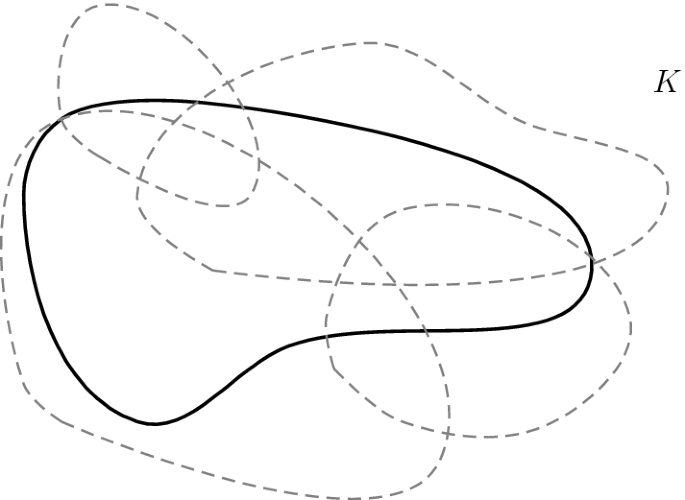
\includegraphics[width=0.4\textwidth]{pictures/ueberdeckung}
\caption{Offene Überdeckung der Menge $K$ \cite{Überdeckung}}
\end{figure}
\begin{bsp}
Wir schauen uns hierzu eine Überdeckung des $\R^2$ an. Wir nennen $\mathcal{U} = \bigcup\limits_{i \in I}{U_i}$ die Familie offener Überdeckungen und definieren $\mathcal{U} = \{B_1(m,n)\: | \: m.n \in \Z\}$.
\begin{figure}[h]
\centering
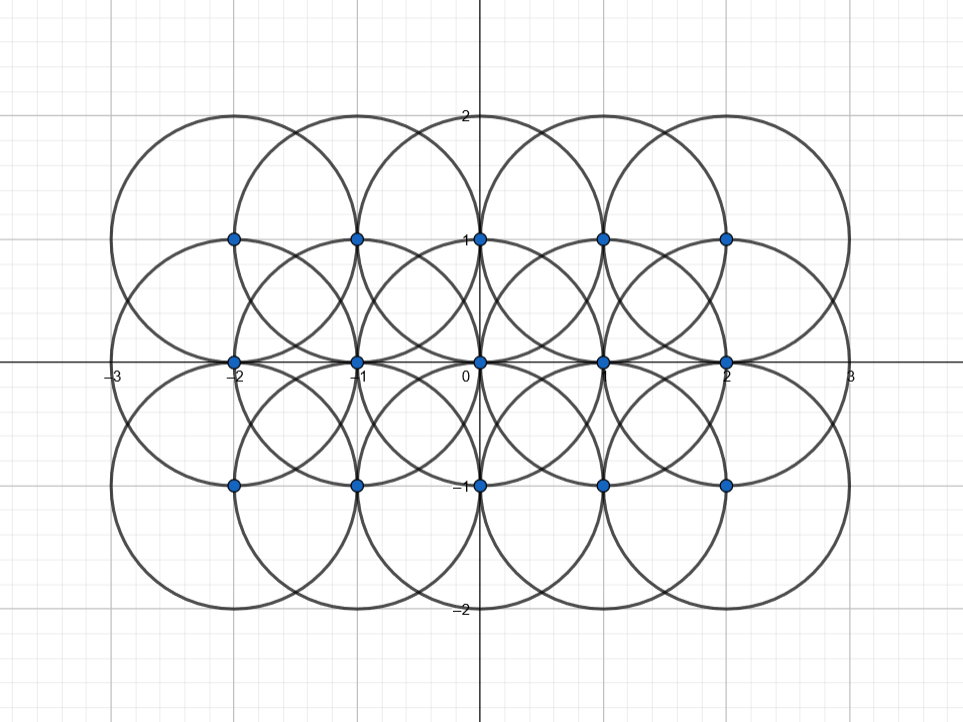
\includegraphics[width=0.50\textwidth]{pictures/ueberdeckung-R2}
\caption{Überdeckung des $\R^2$ (Ausschnitt)}
\end{figure}
\quad\\
Als Beispiel für eine endliche Teilüberdeckung betrachten wir das kompakte Intervall K = [0,1]. $T$ ist eine Teilüberdeckung von $\mathcal{U}= \bigcup_{i \in I}{U_i}$, wenn $T \subset \mathcal{U}$ ist und ebenso $K$ abdeckt. Wir können $K$ mit der Familie $\mathcal{U} = \{(-1,1),(0,2),(1,3)\}$ offener Mengen abdecken. Offensichtlich gibt es aber eine Teilüberdeckung  $T = \{(-1,1),(0,2)\}$, die Teilmenge von $\mathcal{U}$ ist und auch $K$ abdeckt. Hat eine solche Menge endlich viele Elemente, dann nennt man sie eine endliche Teilüberdeckung.
\end{bsp}
\begin{dfi}
(vgl. Ref. \cite{Clason}, S.11) $K \subset X$ heißt \textit{folgenkompakt}, falls jede Folge in $K$ eine konvergente Teilfolge besitzt, die in $K$ konvergiert.
\end{dfi}
\begin{bsp}
Schauen wir uns hierzu ein Gegenbeispiel an. Sei $K = \{\frac{1}{n} \:| \: n \in \N\} = \{1, \frac{1}{2}, \frac{1}{3}, ...\}$, dann konvergiert die Folge $\frac{1}{n}$  gegen $\lim_{n \to \infty}{\frac{1}{n}} = 0 \notin K$. Somit ist die Menge nicht folgenkompakt.
\end{bsp}
\begin{dfi}
(vgl. Ref. \cite{Clason}, S.11) $K \subset X$ heißt \textit{totalbeschränkt}, falls für alle $\epsilon > 0$ eine endliche Überdeckung mit offenen Kugeln existiert, d.h es existiert eine Menge von Punkten $x_1, ..., x_N \in K$ \\($\epsilon$-Netz), sodass gilt:
\begin{align*} 
K \subset \bigcup_{n=1}^{N}{U_\epsilon(x_n)}
\end{align*} 
\end{dfi}
\begin{bem}
Dieser Begriff wird auch oft als Präkompaktheit bezeichnet. Wir werden sehen, dass uns dieser Begriff ermöglicht den Satz von Heine-Borel zu verallgemeinern.
\end{bem}
In metrischen Räumen gelten sogar folgende Äquivalenzen.
\begin{sa}
\label{komp_eq}
(vgl. Ref. \cite{Clason}, S.12) Für $K \subset X$ sind äquivalent:
\begin{itemize}
\item[(i)] $K$ ist kompakt
\item[(ii)] $K$ ist folgenkompakt
\item[(iii)] $K$ ist vollständig und totalbeschränkt
\end{itemize}
\end{sa}
\begin{bem}
Für den Beweis dieser Äquivalenzeigenschaften siehe (Ref. \cite{Clason}, S.12).
\end{bem}
\noindent Ist $(K,d)$ ein metrischer Raum und K kompakt, spricht man auch von einem \textit{kompakten Raum}.
\begin{figure}[h]
\centering
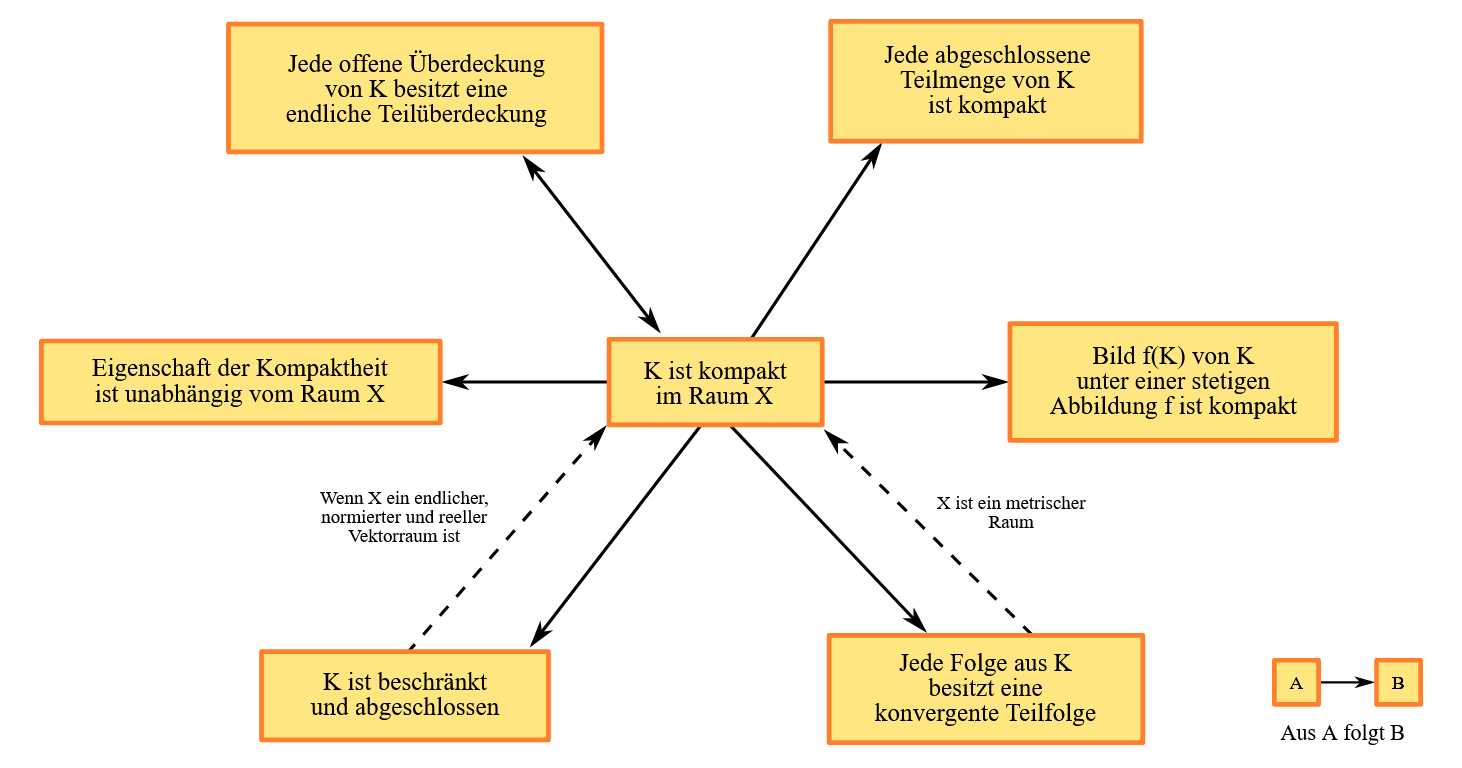
\includegraphics[width=0.95\textwidth]{pictures/kompaktheit.png}
\caption{Eigenschaften kompakter Mengen \cite{KompakterRaum}}
\end{figure}
\quad\\
Bevor wir uns die Beziehung \glqq$K$ ist kompakt $\Leftrightarrow$ K ist beschränkt und abgeschlossen\grqq $\:$genauer anschauen, benötigen wir zwei wichtige Lemmata, die uns wichtige Zusammenhänge zwischen kompakten und abgeschlossenen Mengen herstellen.
\begin{lem}
\label{a}
(Ref. \cite{Clason}, S.13) Ist $K \subset X$ kompakt und $C \subset K$ abgeschlossen, dann ist auch C kompakt.
\end{lem}
\begin{bew}
Seien $K \subset X$ kompakt und $C \subset K$ eine abgeschlossene Teilmenge. Desweiteren sei $(U_i)_{i \in I}$ eine offene Überdeckung von $C$. Wir suchen eine endliche Teilüberdeckung.\\
Durch Hinzunahme der offenen Menge $U = X \setminus C$ erhalten wir eine offene Überdeckung von $K$. Da $K$ kompakt ist, gibt es eine endliche Teilmenge $E \subset I$ mit 
\begin{align*}
K\subset U \cup \bigcup_{k \in E }{U_k}
\end{align*}
Wegen $C \cap U = \emptyset$ ist dann aber
\begin{align*}
C \subset U \cup \bigcup_{k \in E }{U_k}
\end{align*}
und wir haben für $C$ eine endliche Teilüberdeckung von $(U_i)_{i \in I}$ gefunden. (Ref. \cite{tu}, S.24)
\end{bew}
\begin{lem}
\label{quader}
(Ref. \cite{tu}, S.22) Seien $I_1, ..., I_n$ abgeschlossene und beschränkte Intervalle in $\R, I_k = [a_k, b_k]$.  Dann ist der abgeschlossene Quader $Q = I_1 \times ... \times I_n$ kompakt.
\end{lem}
\begin{bew}
Sei${(U_i)}_{i \in I}$ eine offene Überdeckung von $Q$. Wir nehmen an, es gäbe keine endliche Teilfamilie von $ {(U_i)}_{i \in I}$, die $Q$ ganz überdeckt.\\\\
Wir zerlegen $Q$ durch Halbieren aller Seiten in $2^n$ abgeschlossene Teilquader vom halben Durchmesser. Dann gibt es wenigstens einen dieser Teilquader, wir nennen ihn $Q_1$, welchen wir nicht durch endlich viele der $U_i$ überdecken können. Auch $Q_1$ zerlegen wir wieder durch Halbieren aller Seiten in $2^n$ abgeschlossene Teilquader vom halben Durchmesser. Dann gibt es auch wieder wenigstens einen Teilquader, wir nennen ihn $Q_2$, den wir nicht durch endlich viele der $U_i$ überdecken können. Durch Fortsetzung dieses Verfahrens finden wir eine Folge von abgeschlossenen Quadern 
\begin{align*}
Q \supset Q_1 \supset Q_2 \supset ...
\end{align*}
\begin{figure}[h]
\centering
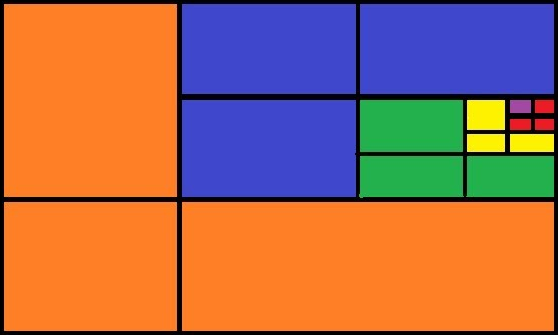
\includegraphics[width=0.35\textwidth]{pictures/heine-borel-theorem}
\caption{Folge von abgeschlossenen Quadern}
\end{figure}
\quad\\
mit diam$Q_k \rightarrow 0$, von denen sich keiner durch endlich viele der $U_i$ überdecken lässt. Nach dem Schachtelungsprinzip gibt es $x \in \bigcap Q_k \subset Q$. Nach Voraussetzung gibt es ein $i_0$ mit $x \in U_{i_0}$. Weil $U_{i_0}$ offen ist, gibt es ein $\epsilon > 0$ mit $U_\epsilon(x) \subset U_{i_0}$. Dann liegt aber jeder Quader $Q_k$ vom Durchmesser $<\epsilon$ ganz in $U_{i_0}$. Das ist ein Widerspruch zu unserer Annahme. (Ref. \cite{tu}, S.22)
\end{bew}
\begin{lem}
(Ref. \cite{Clason}, S.17) Ein kompakter metrischer Raum ist separabel.
\end{lem}
\begin{bem}
Wir wollen uns kurz klar machen, dass die Umkehrung dieses Lemmas nicht gilt. Wir wissen, dass $\R = (-\infty,0) \cup (0, \infty)$ separabel ist. Offensichtlich lässt sich aber keine Kugel mit endlichem Durchmesser um $\R$ legen. Damit ist $\R$ nicht beschränkt und somit auch nicht kompakt.
\end{bem}
\newpage

%%%%%%%%%%%%%%%%%%%%%%%%%%%%%%%%%
%Satz von Heine Borel
%%%%%%%%%%%%%%%%%%%%%%%%%%%%%%%%%
\subsection{Satz von Heine Borel}

\begin{sa}
\label{heine-borel}
(vgl. Ref. \cite{Clason}, S.14) $K \subset \R^n$ ist \textit{kompakt} $\Leftrightarrow$ K ist abgeschlossen und beschränkt
\end{sa}
\begin{bew}
$\Rightarrow$: Diese Richtung folgt direkt aus Satz \hyperref[komp_eq]{\ref*{komp_eq}} und gilt damit sogar allgemein auf jedem metrischen Raum. Die Menge $K$ ist nach Satz \hyperref[komp_eq]{\ref*{komp_eq}} (iii) folgenkompakt und damit beschränkt. mit Satz \hyperref[komp_eq]{\ref*{komp_eq}} (ii) gilt desweiteren, dass jede Folge einen Häufungspunkt in $K$ besitzt. Es liegt also jeder Grenzwert (einziger Häufungspunkt) einer konvergenten Folge in $K$. Damit ist $K$ abgeschlossen.\\\\
$\Leftarrow$: Nehmen wir an, die Menge $K$ sei abgeschlossen und beschränkt. Da die Menge beschränkt ist lässt sich eine Kugel mit endlichem Durchmesser um diese legen, sodass $K \subset B_r(x)$. Da jede Kugel von einem abgeschlossenen Quader $Q$ eingeschlossen werden kann, gilt somit $K \subset B_r(x) \subset Q$. Da nach Lemma \hyperref[quader]{\ref*{quader}} abgeschlossene Quader im $\R^n$ kompakt sind, können wir mit Lemma \hyperref[a]{\ref*{a}} direkt folgern, dass auch $K$ kompakt ist.
\end{bew}
Die Hinrichtung gilt also allgemein auf metrischen Räumen, jedoch die Rückrichtung nur im $\R^n$. Wir wollen uns das klar machen, indem wir einen unendlichdimensionalen Raum betrachten, indem die abgeschlossene Einheitskugel nicht kompakt ist.\\\\
Insbesondere ist mit Satz \hyperref[heine-borel]{\ref*{heine-borel}} die abgeschlossene Einheitskugel
\begin{align*}
B_1(x) = \{x \in \K^n | \|x\|_2 \leq 1\}
\end{align*}
 im euklidischen Raum kompakt.
Betrachten wir nun die abgeschlossene Einheitskugel im Banachraum $(C[0,1], \|\cdot\|_\infty)$:
\begin{align*}
B_1(x) = \{f \in C[0,1] \: | \: \|f\|_\infty \leq 1\}
\end{align*}
Es sei ${(f_k)}_{k \in \N}$ eine Folge von Funktionen $f_k \in (C[0,1], \|\cdot\|_\infty)$. Betrachten wir eine beliebige Teilfolge ${(f_{k_j})}_{j \in \N}$, dann gilt wegen $k_j \neq k_l$ für $j \neq l$ (konstante Folgen ausgeschlossen) auch
\begin{align*}
\|f_{k_j} - f_{k_l}\|_\infty = \max_{x \in [0,1]}{|f_{k_j}(x) - f_{k_l}(x)|} = 1
\end{align*}
für beliebige $j \neq l$. Die Teilfolge ${(f_{k_j})}_{j \in \N}$ ist also keine Cauchy-Folge und besitzt damit keinen Grenzwert in $(C[0,1], \|\cdot\|_\infty)$. Damit ist die abgeschlossene Einheitskugel hier nicht kompakt. (vgl. Ref. \cite{uni})\\\\
Für allgemeine metrische Räume gilt allerdings eine Verallgemeinerung des Satzes.
\begin{sa}
Es sei $(X,d)$ ein vollständiger metrischer Raum und $K \subset X$. Dann gilt:
\begin{align*}
K \: \text{ ist kompakt} \: \Leftrightarrow K \: \text{ist abgeschlossen und totalbeschränkt}
\end{align*}
\end{sa}
\begin{bem}
Dies ist eine Verallgemeinerung von Satz \hyperref[heine-borel]{\ref*{heine-borel}}, da für $A \subset \R^n$ gilt:
\begin{align*}
 A \: \text{ist totalbeschränkt} \: \Leftrightarrow \: A \: \text{ist beschränkt}
\end{align*}
\end{bem}
\newpage

\pagestyle{plain}
%%%%%%%%%%%%%%%%%%%%%%%%%%%%%%%%%%%%%%%%%%%%%%%%%%%%%%%%%%%%%%%%%%
%Abbildungsverzeichnis
%%%%%%%%%%%%%%%%%%%%%%%%%%%%%%%%%%%%%%%%%%%%%%%%%%%%%%%%%%%%%%%%%%
\section*{}
\addcontentsline{toc}{section}{Abbildungsverzeichnis}
\printbibliography[title=Abbildungsverzeichnis, type=misc]

%%%%%%%%%%%%%%%%%%%%%%%%%%%%%%%%%%%%%%%%%%%%%%%%%%%%%%%%%%%%%%%%%%
%Internetquellen
%%%%%%%%%%%%%%%%%%%%%%%%%%%%%%%%%%%%%%%%%%%%%%%%%%%%%%%%%%%%%%%%%%
\section*{}
\addcontentsline{toc}{section}{Internetquellen}
\printbibliography[title=Internetquellen, nottype=book, nottype=misc]

%%%%%%%%%%%%%%%%%%%%%%%%%%%%%%%%%%%%%%%%%%%%%%%%%%%%%%%%%%%%%%%%%%
%Literatur
%%%%%%%%%%%%%%%%%%%%%%%%%%%%%%%%%%%%%%%%%%%%%%%%%%%%%%%%%%%%%%%%%%
\section*{}
\addcontentsline{toc}{section}{Literatur}
\printbibliography[title=Literatur, type=book]



\end{document}
